\chapter{Profiling Contur}
\label{chapterlabel3}
An important part of the task of optimising contur is to first perform a profile of the code. This section will outline the steps taken to produce a profile of contur and how the results were used. We will start by introducing cProfile, which is the Python profiler which was used to carry out the profile. Then we will discuss Snakeviz and gprof2dot, these are the two tools which we used to visualize the profiling results produced by cProfile. Finally we will conclude the section by performing an initial profile of the contur package before any code optimization was attempted. This initial profile will serve as our benchmark to measure the effectiveness of our later attempts to improve the run time performance of contur.

\section{Profiling with cProfile}

\subsection{Why cProfile?}
Let us first begin by considering some of the features we ideally require from our chosen profiler. At a minimum a profiler must obviously be able to time how long it takes our code to run. This basic requirement is essential to be able to determine if our attempted improvements to the code do in fact actually improve run performance. In addition to just providing the total run time of contur we will also require our profiler to provide a split of the runtime among the functions/sub-functions which compose contur. A split of the run time like this will highlight parts of the code that consume disproportionately large amounts of CPU or are repetitively called, suggesting optimisation improvements can be made.

cProfile is a module within the Python standard library which meets these requirements. Our main motivations for using cProfile are as follows:

\begin{itemize}
\item Provides a full profile of program with output include total run time, time taken at each individual step, and number of calls to individual functions;
\item Easy to save the output of the profile in prof files which can then be read by tools built to visualize profiling results;
\item Performing the profile with cProfile is quick and easy and requires minimal new code;
\end{itemize}

\subsection{Using cProfile}
The last version of contur which exists in the main contur repository before any optimisation changes were attempted can be found at commit \href{https://gitlab.com/hepcedar/contur/-/tree/49a67e039cf93c88b39dade3dfb7c5f03e780fb2}{49a67e03}. In this section we will walk through the steps required to profile this version of contur running on a single yoda file. The steps required to perform the profile on a contur grid run are the same, so the in the next section we will just provide the results for a grid run of this version of contur.

The simplest way of performing a profile with cProfile is via cProfile's run method. To profile contur using the run method we just pass contur's main function to the run method. We can make this adjustment to contur's code by updating the main run script \href{https://gitlab.com/hepcedar/contur/-/blob/master/bin/contur}{here} as follows 

\begin{minted}{python}

import cProfile

if __name__ == "__main__":
       cls_args = get_args(sys.argv[1:],'analysis')
       cProfile.run("main(cl_args)", sort=cumtime) #perform profile
       
\end{minted}

After updating the run script as above we can now run contur as normal to get the below terminal output from the profile

\begin{figure}[H]
\centering
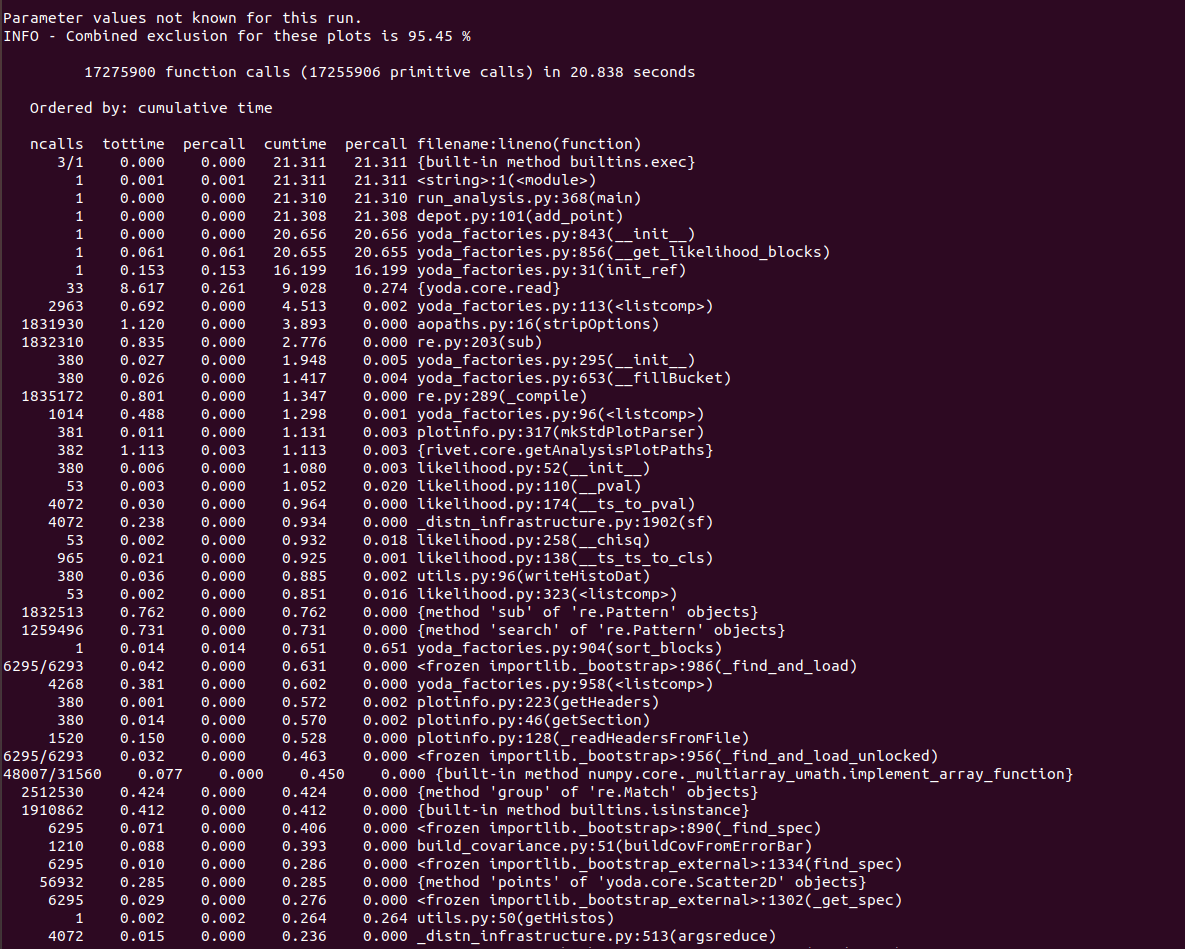
\includegraphics[scale=0.35]{plots/example_profile.png}
\caption{Output of cProfile run method}
\label{fig:ep}
\end{figure}

From figure \ref{fig:ep} above we can summarise the main output from the single yoda file contur run:

\begin{itemize}
\item From line one of the profiling results we can see that the run had c.a. 17 million function calls and took c.a. 20 seconds to run;
\item The next line tells us that we are ordering the profiling results by cumulative time (cumtime column). The cumulative time for a function is the time spent to run a function and all other functions called within the function (so the cumtime for the main function will be the total run time of the program as all other functions are called within main);
\item From line three on we have the profiling information for the functions and sub-functions which compose the contur run. The main columns which stand out here are 'ncalls' which gives the number of calls made to the function, 'tottime' which gives the total time spent in the function excluding calls to sub functions and finally 'cumtime' which as already explained gives the run time for each function including all the calls to sub functions.;
\end{itemize}

The above profiling is already useful, it gives us things like the run time and the break down of the run time between the components of contur. However the printed results in the current form are not very readable, a detailed knowledge of the functions that compose contur would be needed to take any advantage of the run time broken down by components in its current form. Additionally we don't just want to print result to the terminal and work from there, we would preferable save the profiling results to some file format so our results are reusable across time. 

To meet both these objectives for the profiling we  from here on we will print the data from our profile into '.prof' files which can then be read by tools which help visualise the profiling results. We do this by introducing the Profile class of cProfile and using this to perform our profiles from here on in as opposed to using the run method, the updated code to perform the profiling with the Profile class is given below.

\begin{minted}{python}

import cProfile, pstats, io

if __name__ == "__main__":
       cls_args = get_args(sys.argv[1:],'analysis')
       
       pr = cProfile.Profile()
       pr.enable()
       
       main(cl_args)
       
       pr.disable()
       pr.dump_stats('outfile.prof'')
\end{minted}


\section{Visualizing Profiling Results}

To visualise our profiling results we will use two open source tools Snakeviz and gprof2dot. As what follows will show, we can use both of these tools in a complementary way, as opposed to a simple choose of one or the other, to help make best of use of the profiling data we produce with cProfile.

\subsection{Snakeviz}
Snakeviz is a browser based graphical viewer for the output of Python's cProfile profiler module. Snakeviz can easily be pip installed with the following terminal command

\begin{lstlisting}[language=bash]
  $ pip install snakeviz
\end{lstlisting}

once installed we can invoke snakeviz to visualise an arbitrary .prof file as follows

\begin{lstlisting}[language=bash]
  $ snakeviz profile_file.prof
\end{lstlisting}

After invoking snakeviz as outlined above the web browser interface for the tool will open and the user can explore the profiling results. Snakeviz allows user interaction to adjust how results are rendered, the two main plotting options available in Snakeviz are icicle plots and sunburst plots. From here on we will use Snakeviz's icicle plot to explore profiling results, additionally due to the constraints of the static form this document is written in we will just examine static snapshots of the overall display in Snakeviz's viewer. These static snapshots of the Snakeviz viewer are sufficient to summarise profiling results, using Snakeviz's viewers ability to adjust rendering though can be useful to get a feel and understanding for new profiling results, the interested reader is recommended to play around with Snakeviz's viewer functionality further.

Below in figure \ref{fig:single_yoda_start_profile_snakeviz} we show a snapshot of an icicle plot from a profile of our initial starting contur code on a single yoda file. From the figure we can seen that the icicle plot is showing the same information as figure \ref{fig:ep} in just a more visually appealing way, with the addition that in the icicle plot we can see the ordering of the calls to the components of code that compose a contur run. This ordering is very useful additional information, for example from the ordering it jumps out at us that the call to yoda.core to read the yoda passed to contur takes a large proportion of the run time for a single contur run. From this we can already understand that a lot of the run time for a single contur run comes from just reading in data. 

\begin{figure}[H]
\centering
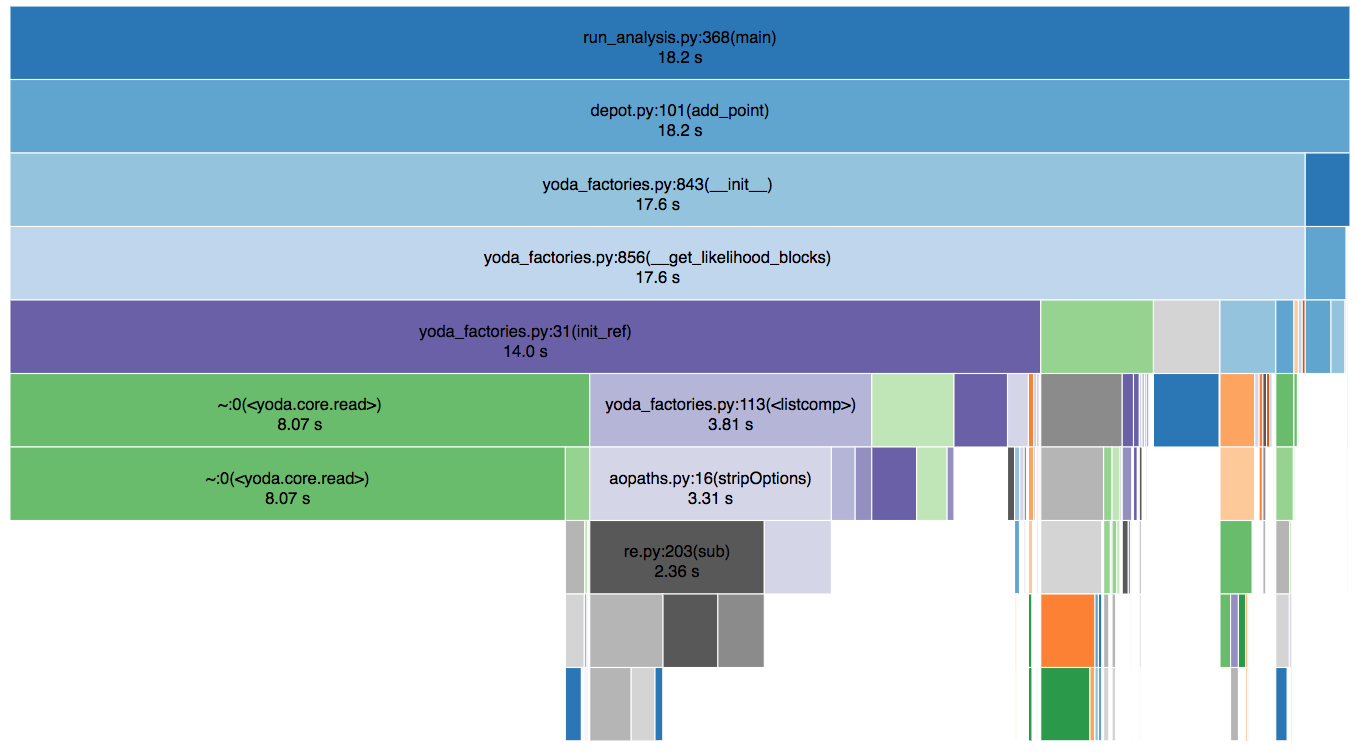
\includegraphics[scale=0.3]{plots/initial_single_contur.png}
\caption{Contur single yoda run starting point - Example snakeviz icicle plot}
\label{fig:single_yoda_start_profile_snakeviz}
\end{figure}

\subsection{gprof2dot}
gprof2dot is a python script that converts the output of the cProfile to dot plots. These dot plots can be used to complement the information we get from the icicle plots. The icicle plots and the user interface offered by snakeviz offer a means to see the absolute run of our code and how this absolute run time breaks down among the components of the program. The dot plot complement complements this information by providing a rendering which makes the flow of the code (i.e. the progression of the code from the call to main through the components that compose the program) more easily visible and additionally showing the relative weight run time wise of the components of the code. This visualisation can be useful to both quickly spot bottlenecks in the code and also just to get a better understand of how a large code base works.

\begin{figure}[H]
\centering
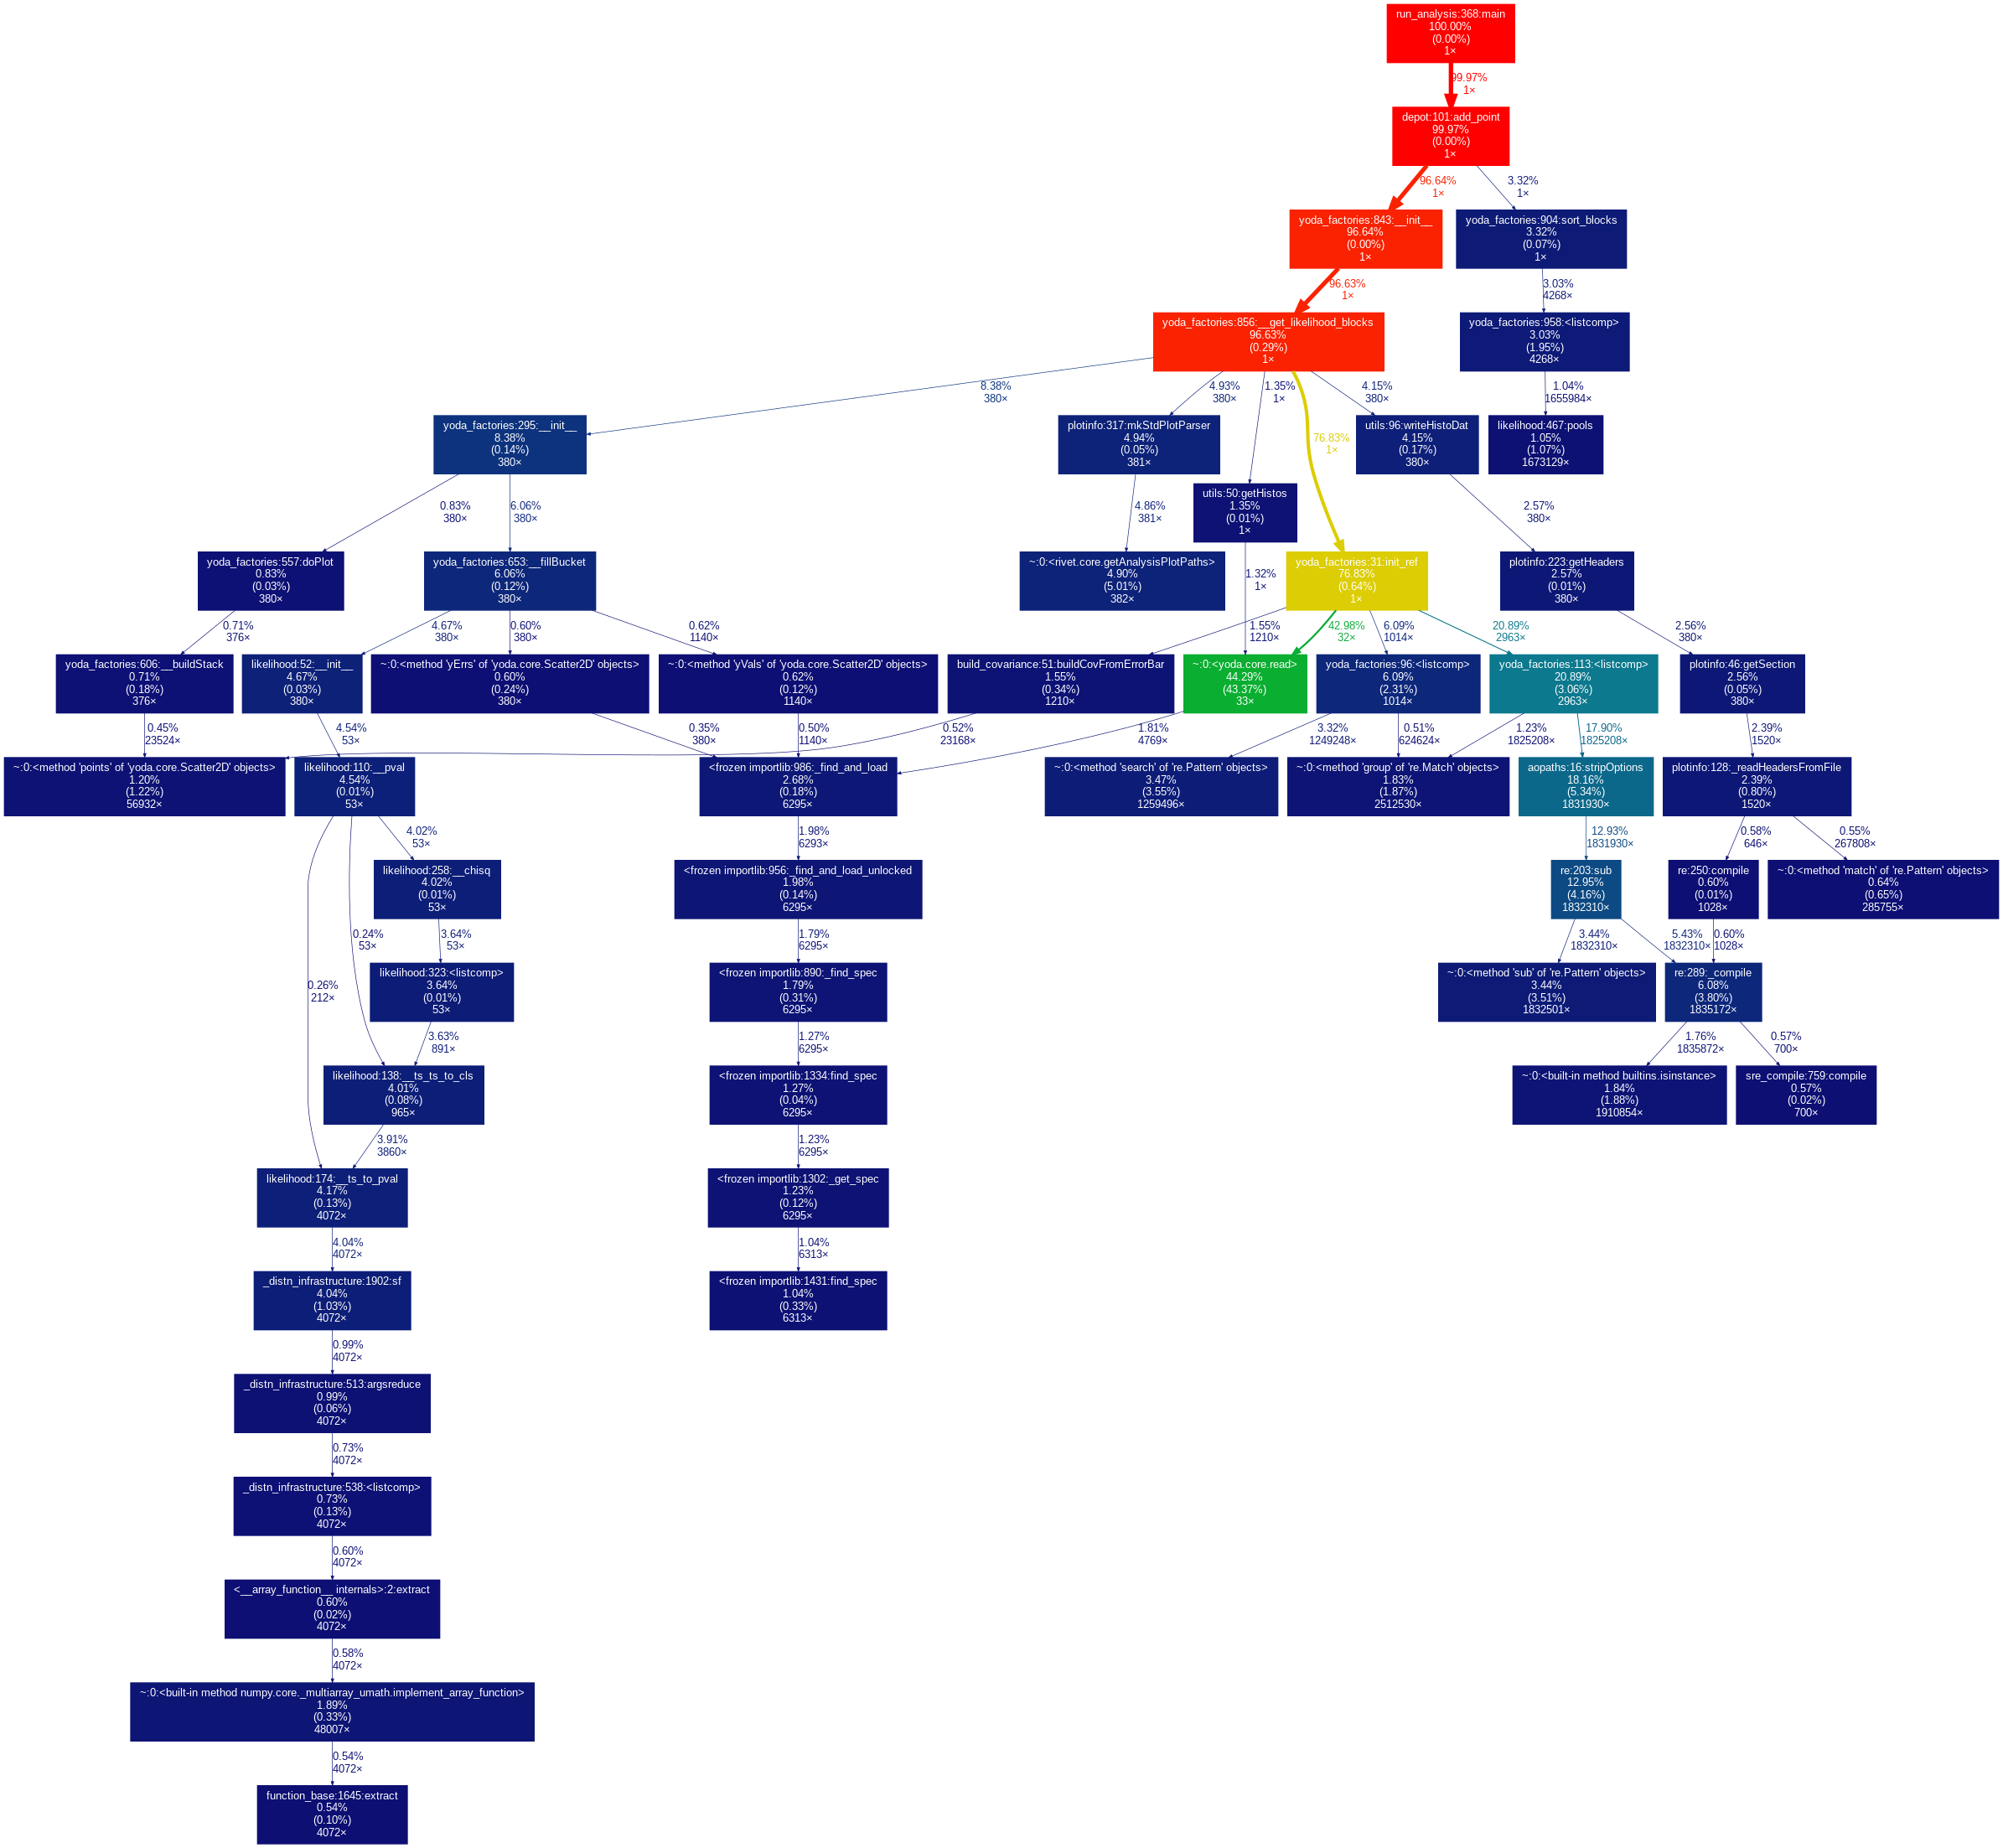
\includegraphics[scale=0.2]{plots/initial_contur_single_yoda.png}
\caption{Contur single yoda run starting point - Example gprof2dot}
\label{fig:single_yoda_start_profile_gprof2dot}
\end{figure}

We can see example of the dot plots produced by gprof2dot in figure \ref{fig:single_yoda_start_profile_gprof2dot} above. This plot is visualising the same single yoda contur run as in figure \ref{fig:single_yoda_start_profile_snakeviz}, so is a good way of demonstrating the complementary nature of the icicle plot and the dot plots for visualising our profiling results. Following the coloring scheme in the dot plot (red to yellow to green) the observation we previously made using the icicle plot about the weight of data reading in the run time can be seen in the dot plot where we can see c.a. $42\%$ of run time is spent reading yoda files.

\section{Initial Profile Results}
In the previous section while introducing the visualisation tools we gave the initial profiling results resulting from running contur on a single yoda file (see figure \ref{fig:single_yoda_start_profile_snakeviz} and \ref{fig:single_yoda_start_profile_gprof2dot} ) before any optimisation of the code was attempted. As previously discussed, in practical settings contur is generally run on a grid of yoda files as opposed to a single yoda file, so along with our initial single yoda run profile we will also perform an initial profile of contur on a test grid. The grid we use to perform this profile is a $10 \times 10 $ grid, so composed of $100$ yoda files in total, we will use this reference grid through out to profile contur's grid run.

In figure \ref{fig:grid_yoda_start_profile} below we see the icicle plot for the grid run, from this we can see that for the grid of 100 yoda files we have a run time of around $1100$ seconds or close to $20$ minutes. 
\begin{figure}[H]
\centering
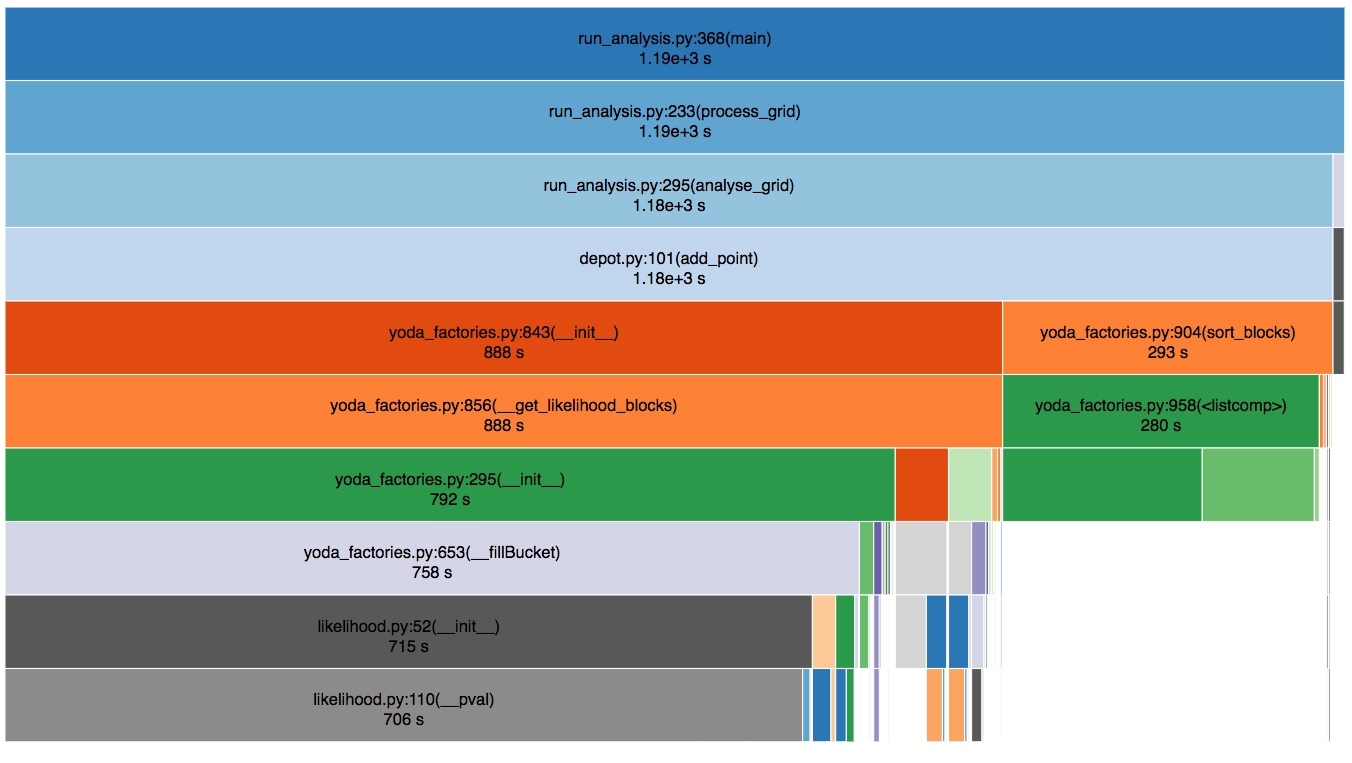
\includegraphics[scale=0.30]{plots/initial_contur_grid_profile_two.png}
\caption{Contur grid run - icicle plot}
\label{fig:grid_yoda_start_profile}
\end{figure}

We can also see from the plot that the main contribution to the run time seems to be coming from two blocks of the code. This is best seen in the dot plot figure \ref{fig:grid_yoda_start_profile_dot} below where we can see that the sort blocks method contributes c.a. $25\%$ of the run and the ts to pval method which contributes c.a. $49\%$, so both of these methods in combination are close to three quarters of the run time for the contur grid run.


\begin{figure}[H]
\centering
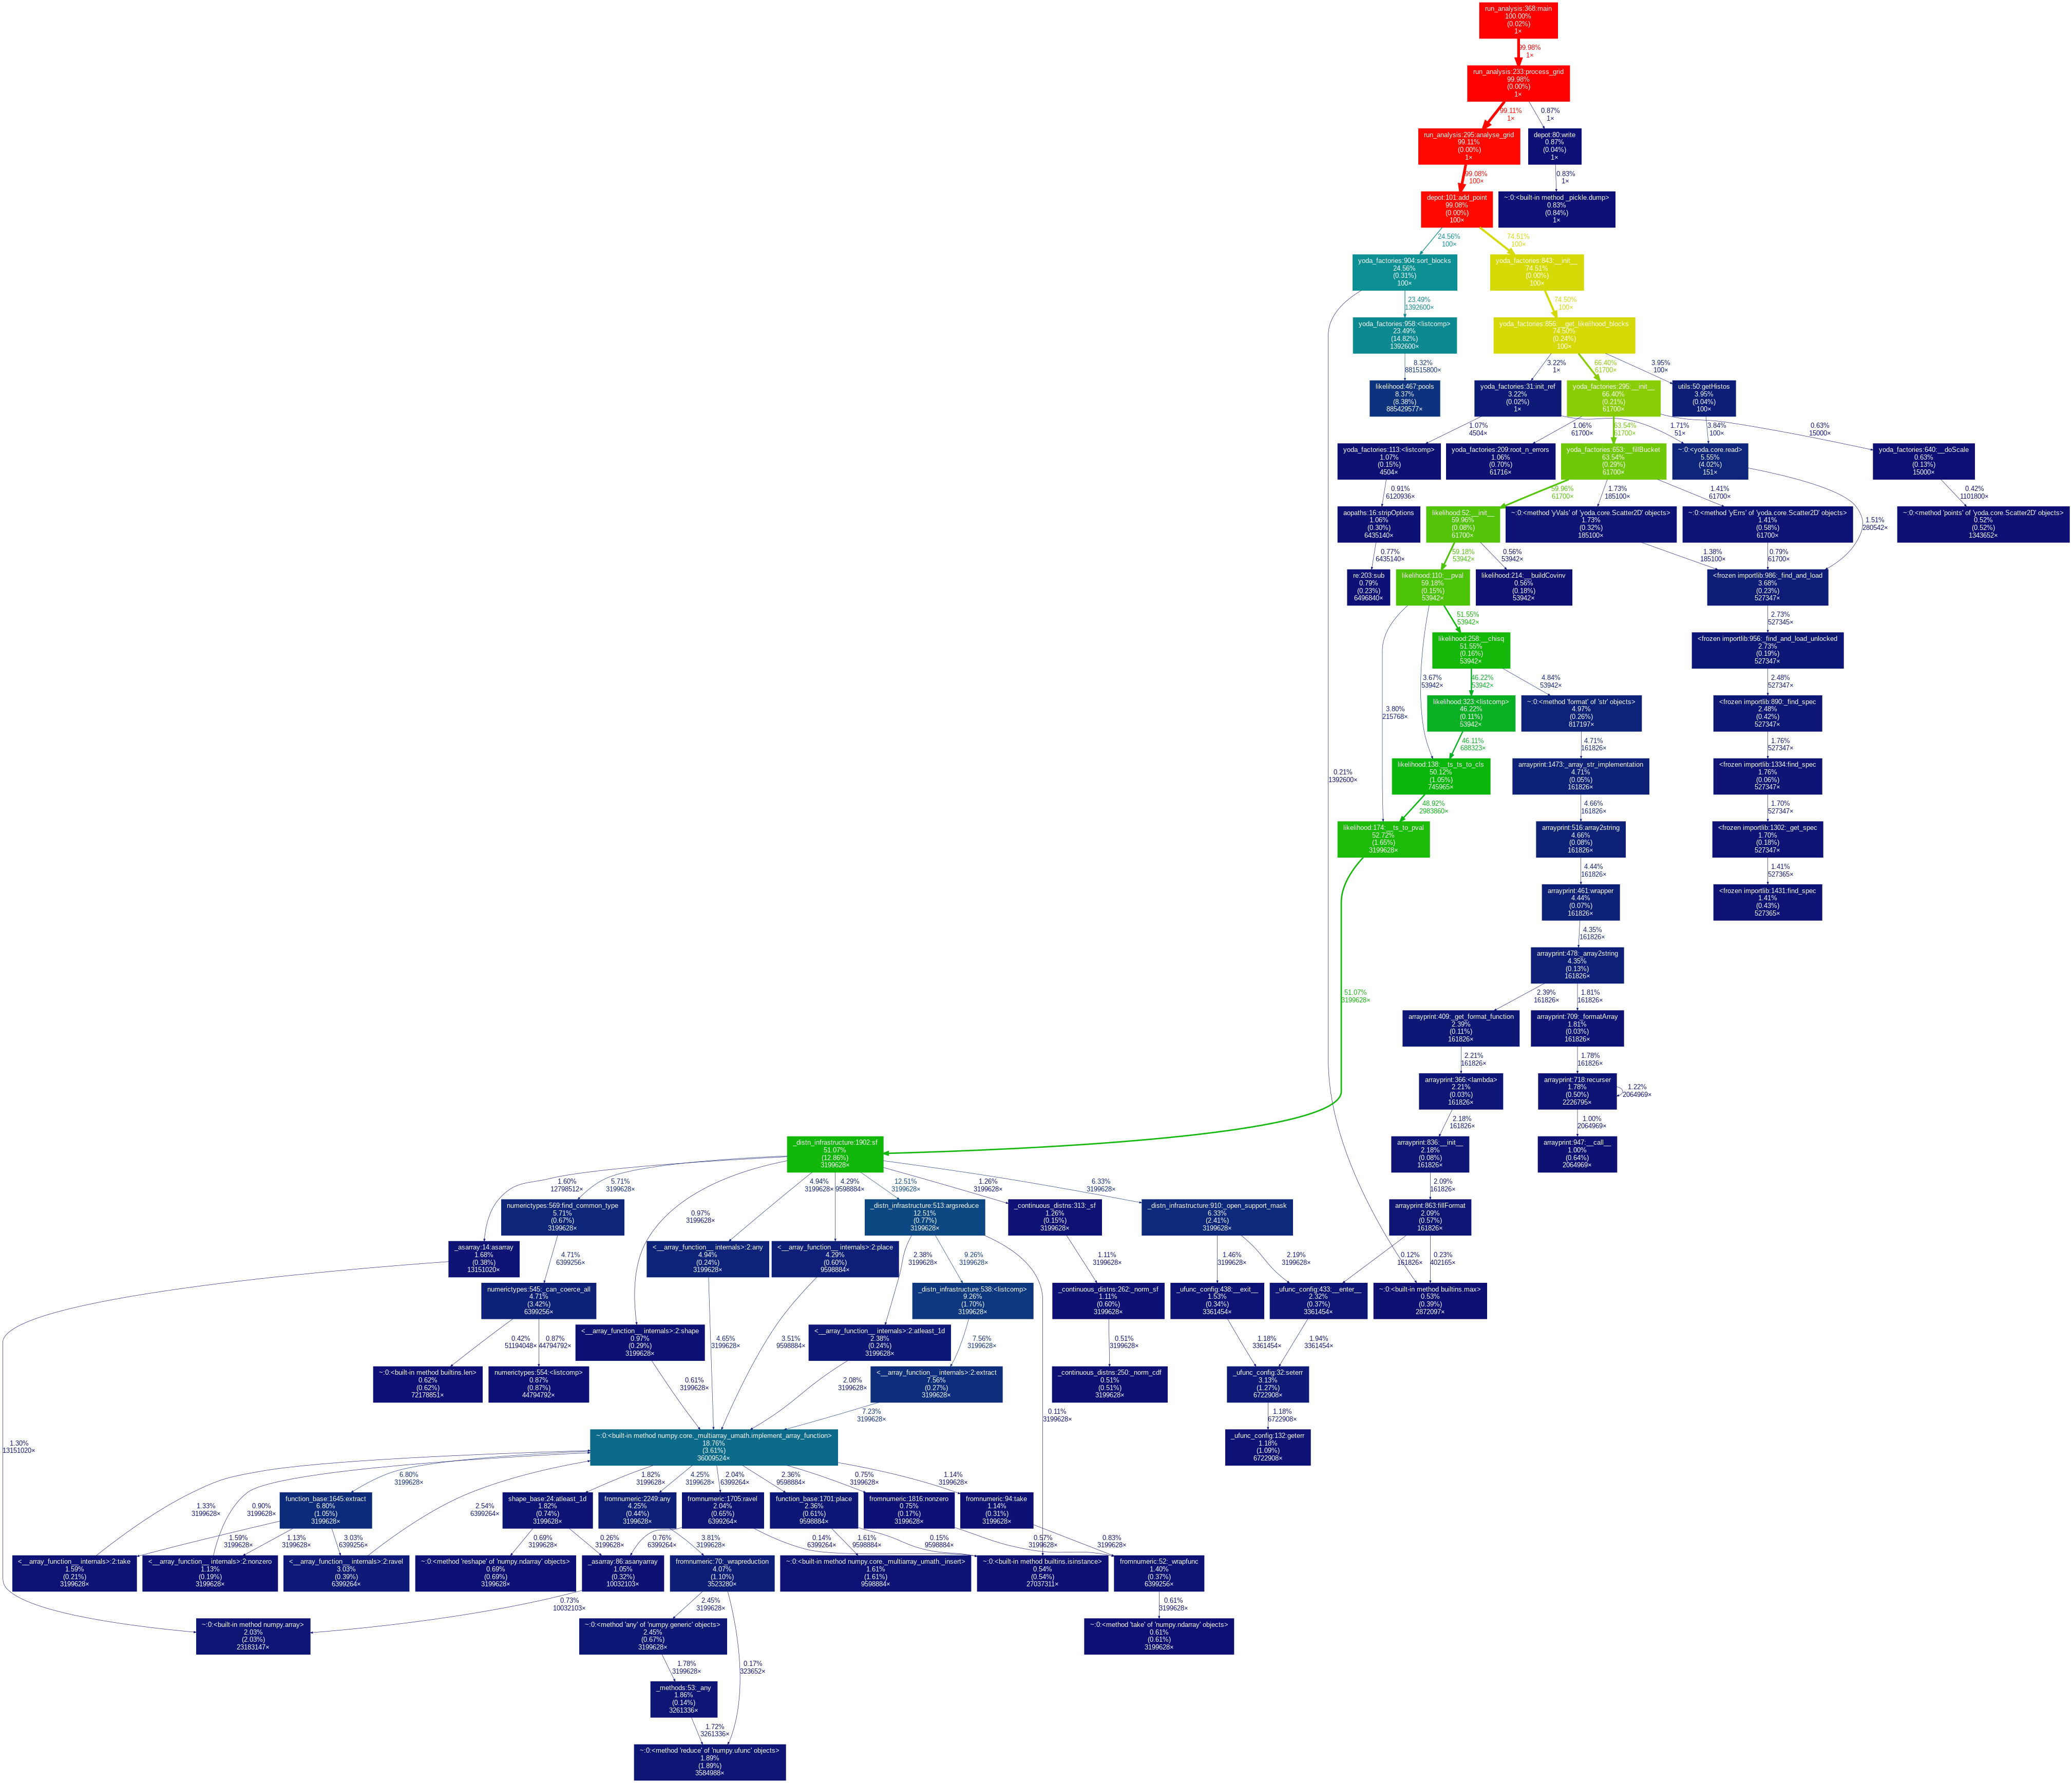
\includegraphics[scale=0.1]{plots/initial_contur_grid_two.png}
\caption{Contur grid run - dot plot}
\label{fig:grid_yoda_start_profile_dot}
\end{figure}




